\begin{frame}
\frametitle{Problem setup: We model the ultrasound-alveolar interaction as a 2D, compressible, inviscid fluid system.}
  \begin{figure}
    \centering
    \begin{subfigure}[b]{0.48\textwidth}
      \phantomcaption \centering \def\svgwidth{\textwidth}
      % \import{./figs/avpaper_figs/}{Alveolus_US_zoom_only_diagram.pdf_tex}
      % \hfill%
      \import{./figs/}{Alveolus_US_tissue_diagram_20170925.pdf_tex}
      \hfill%
      \label{fig:alveolar_schematic}% Physical problem of interest: an \ac{US} wave impinges upon an alveolus.}
    \end{subfigure}
    ~
    \begin{subfigure}[b]{0.48\textwidth}
      \centering \phantomcaption \def\svgwidth{\textwidth}
      % \import{./figs/avpaper_figs/}{usbe_model_schematic_domain.pdf_tex}
      % \hfill%
      \import{./figs/}{usbe_model_schematic_interface_20170915.pdf_tex}
      \hfill%
      \label{fig:problem_schematic}% A schematic of the domain and model problem.}
    \end{subfigure}
  \end{figure}
\end{frame}
% \begin{frame} \frametitle{Problem setup: We model the ultrasound-alveolar interaction as a 2D, compressible, inviscid fluid system.}
%   \begin{figure}
%     \centering
%     \def\svgwidth{0.48\textwidth}
%     {\footnotesize
%       \import{../figs/lung_figs/}{usbe_lung_schematic2.pdf_tex} \hfill%
%     }
%     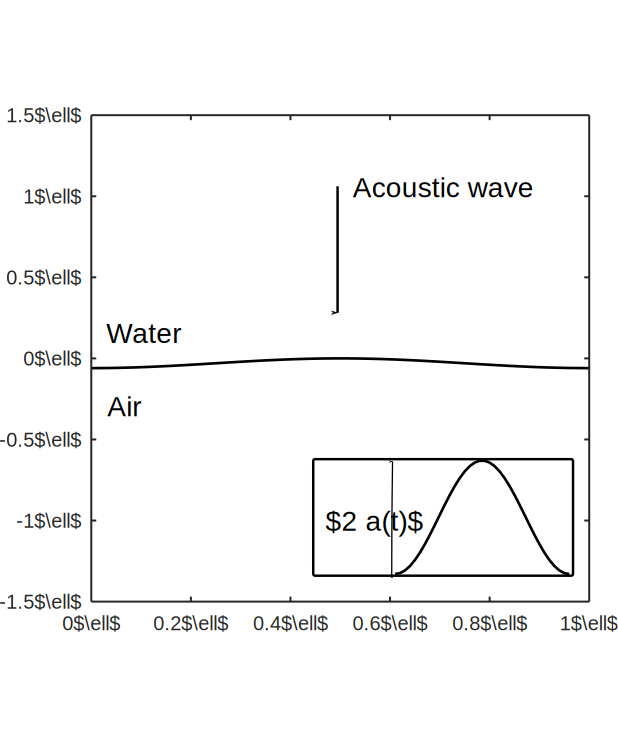
\includegraphics[width=0.48\textwidth]{../figs/lung_figs/usbe_model_schematic} \hfill
%   \end{figure}
%   An acoustic wave impinges downward from water toward a perturbed air interface $(a_0\equals0.06\lambda)$.
%   \note{
%     \begin{enumerate}
%     \item We model an acoustic wave impinging downward from tissue (liquid) onto an air inside an alveolus.
%     \item We use an initially sinusoidal interface with a wavelength $\lambda$, which is the width of our domain. 
%     \item And a peak-to-peak perturbation amplitude of $0.06\lambda$
%     \end{enumerate}
%     }
% \end{frame}


%%% Local Variables:
%%% mode: latex
%%% TeX-master: "../main"
%%% End:
